% Séquence 2 : Points et droites
\setseqtitle{Points et droites}
\chapter{Points et droites}
\label{chap:seq02}

% ======= Petits outils locaux (utilisables dans tout le chapitre) =======
% Pointillés pour les réponses (remplace \underline{\hspace{...}})
\newcommand{\trou}[1]{\makebox[#1]{\dotfill}}
% Styles TikZ (si déjà définis dans le préambule, ces lignes n'ont pas d'effet néfaste)
\tikzset{
	pt/.style   ={circle,fill=black,inner sep=1.2pt},
	lbl/.style  ={font=\footnotesize, inner sep=1pt},
	seg/.style  ={line width=0.9pt},
	dro/.style  ={line width=0.9pt},
	para/.style ={line width=0.9pt, dashed}
}

\begin{objectifsbox}
	\textbf{Vocabulaire et notations :} point, segment, demi-droite, droite, lectures [AB], (AB), [AB), AB.\\
	\textbf{Relations :} appartenance, alignement, droites sécantes/perpendiculaires/parallèles.\\
	\textbf{Méthodes :} tracer des parallèles et des perpendiculaires (règle + équerre).
\end{objectifsbox}

% =========================
\section{ Vocabulaire et notations}
\begin{itemize}
	\item Un point est un lieu dans le plan ; on le nomme par une \trou{5cm} majuscule.
	\item Une droite est une \trou{3cm} définie par \trou{3cm} points distincts ; elle est \trou{3cm} (s'étend à l'infini).
	La droite passant par $A$ et $B$ se note : \trou{5cm}.
	\item Un \trou{3cm} est une portion de \trou{3cm} délimitée par deux \trou{3cm} appelés \trou{3cm}.
	On le note : \trou{3cm}.
	\item Une \trou{3cm} est une partie de \trou{2.2cm} qui commence en un \trou{3cm} donné et s'étend à l'infini.
	On la note par exemple : \trou{3cm}.
\end{itemize}

\textbf{Lecture :} \\
$[AB]$ se lit << \trou{14cm} >> ;\\
$(AB)$ se lit << \trou{14cm} >> ;\\
$[AB)$ se lit << \trou{14cm} >> ;\\
$AB$ se lit << \trou{14cm} >>\\
(ou << \trou{14cm} >>).

% --- Figure vocabulaire : droite, segment, demi-droite, longueur AB
\begin{figure}[h]
	\centering
	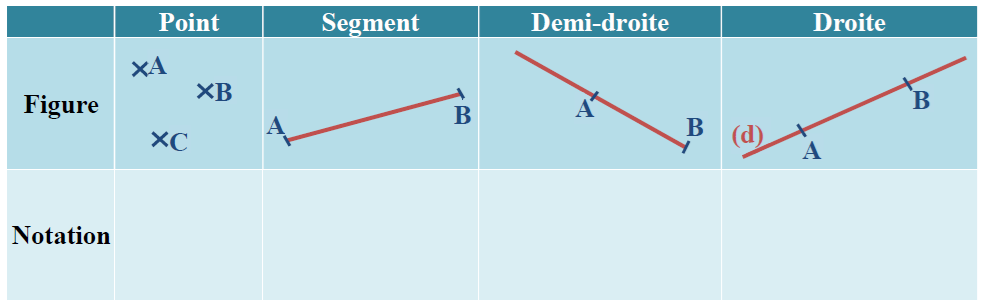
\includegraphics[width=1\linewidth]{../../assets/images/6e/seq_02/points_segment_droites}
	\caption{Vocabulaire : $(AB)$ droite ; $[CD]$ segment ; $[EF)$ demi-droite ; $AB$ longueur.}
	\label{fig:vocab-points-droites}
\end{figure}

\newpage
% =========================
\section{ Appartenance et alignement}

% --- Figure appartenance et alignement
\begin{figure}[h]
	\centering
	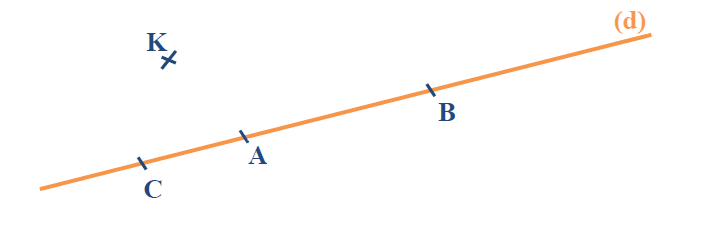
\includegraphics[width=1\linewidth]{../../assets/images/6e/seq_02/pt_sur_dte}
	
	\label{fig:point-sur-droite}
\end{figure}

\begin{definitionbox}
\begin{itemize}[label = \textbullet]
	\item Les points $A$, $B$ et $C$ \textbf{appartiennent} à la droite $(d)$.\\
	On note $A$ \trou{1cm} $(d)$, $B$ \trou{1cm} $(d)$, $C$ \trou{1cm} $(d)$.
	\item Le point $K$ \textbf{n'appartient pas} à la droite $d$. \\
	On note $K$ \trou{1cm} $(d)$
	\item Des points sont dits \textbf{alignés} s'ils \trou{6cm}.
\end{itemize}

\end{definitionbox}

% =========================
\section{ Positions relatives des droites}
\begin{itemize}
	\item Deux droites sont \textbf{sécantes} si elles se coupent en \trou{1.2cm} point.
	\item Deux droites $(d)$ et $d^{\prime}$ sont \textbf{perpendiculaires} si elles se coupent en formant un \trou{1.5cm} \trou{1.5cm}. On note : $(d)\perp(d')$.
	\item Deux droites $(AB)$ et $(EF)$ sont \textbf{parallèles} si elles ne sont pas \trou{5cm}. On note : $(AB) \trous{1.5cm} (EF)$.
\end{itemize}

\textbf{Lecture :} $(AB)//(EF)$ se lit << \trou{8cm} >> (ou << \trou{8cm} >>). \quad $(d)\perp(\Delta)$ se lit << \trou{8cm} >>.

% --- Figures sécantes / perpendiculaires / parallèles
\begin{figure}[h]
	\centering
	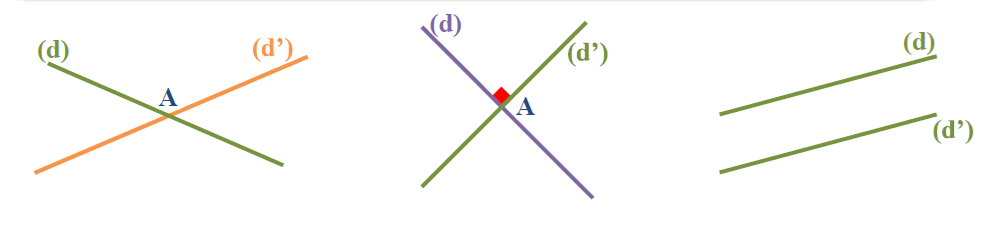
\includegraphics[width=1\linewidth]{../../assets/images/6e/seq_02/position_relative}
	%\caption{Vocabulaire : $(AB)$ droite ; $[CD]$ segment ; $[EF)$ demi-droite ; $AB$ longueur.}
	\label{fig:Position relative de droites}
\end{figure}

% =========================
\section{ Tracer à la règle et à l'équerre}
\begin{itemize}
	\item La perpendiculaire à $(d)$ passant par $A$.
	\item La perpendiculaire à $(d)$ passant B.
	\item La perpendiculaire à $(d)$ passant C.
	\item Coder la figure.
\end{itemize}

% --- Figures de construction : perpendiculaire en A, parallèle par B
\begin{center}
	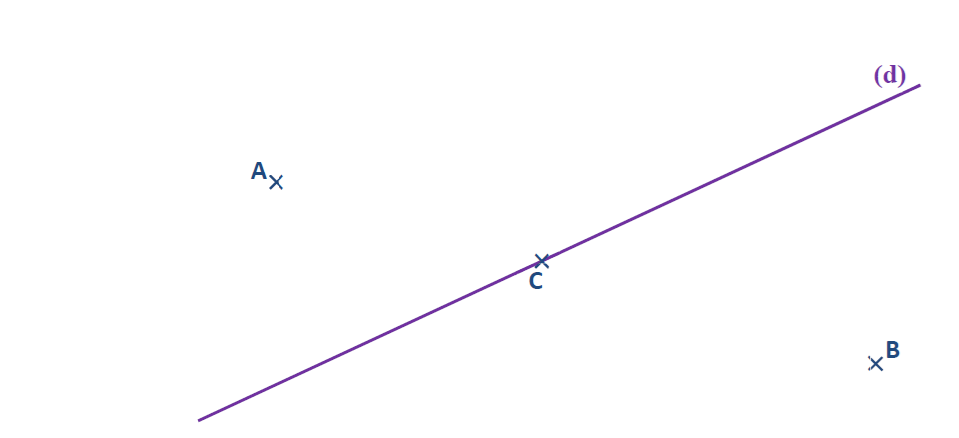
\includegraphics[width=1\linewidth]{../../assets/images/6e/seq_02/ex1}
\end{center}


\begin{itemize}
	\item La parallèle à $(d_1)$ passant par D.
	\item La parallèle à $(d_2)$ passant E.
	\item La parallèle à $(d_1)$ passant F.
	\item La parallèle à $(d_2)$ passant F.
\end{itemize}

\begin{center}
	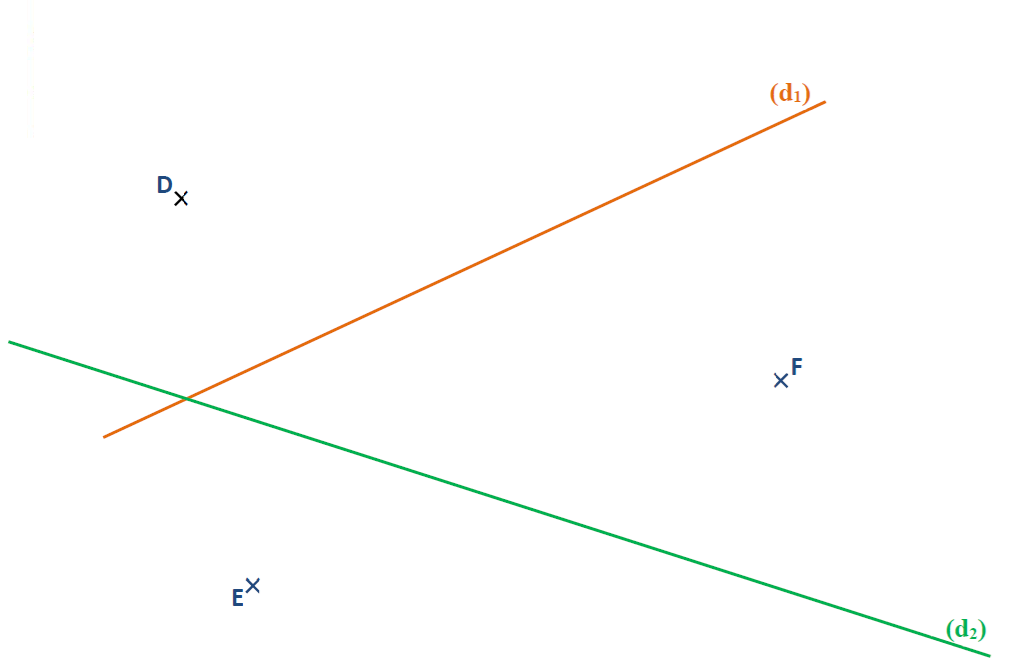
\includegraphics[width=1\linewidth]{../../assets/images/6e/seq_02/ex2}
\end{center}


% =========================
\section{ Propriétés fondamentales des droites}

\noindent % Pour éviter l'indentation du premier paragraphe
En géométrie, il y a des règles de base qui sont toujours vraies. 
En voici trois très importantes à connaître par cœur.

\begin{proprietebox}[La droite passant par deux points]
Par deux points distincts \textbf{A} et \textbf{B}, il ne passe qu'\textbf{une seule et unique droite}.\\
On la note \textbf{(AB)} ou \textbf{(BA)}.
\vspace{0.5cm}
\begin{center}
	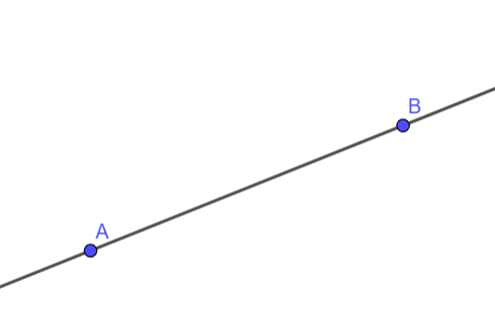
\includegraphics[width=0.5\linewidth]{../../assets/images/6e/seq_02/point_droite}
\end{center}
\textit{Cette règle signifie qu'on ne peut pas tracer deux droites différentes qui passeraient en même temps par les points A et B.}
\end{proprietebox}

\begin{proprietebox}[La parallèle unique]
Soit une droite $(d)$ et un point \textbf{A} qui \textbf{n'est pas sur} la droite $(d)$.\\
Il n'existe qu'\textbf{une seule droite} qui passe par le point \textbf{A} et qui est \textbf{parallèle} à la droite $(d)$.

\vspace{0.5cm}

\begin{center}
	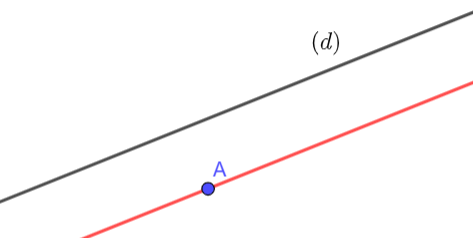
\includegraphics[width=0.5\linewidth]{../../assets/images/6e/seq_02/point_droite_parallele}
\end{center}


\vspace{0.5cm}

\textit{On peut tracer cette droite unique à l'aide d'une règle et d'une équerre.}

\end{proprietebox}

\begin{proprietebox}[La perpendiculaire unique]
Soit une droite $(d)$ et un point \textbf{A} (qu'il soit sur la droite ou non).\\
Il n'existe qu'\textbf{une seule droite} qui passe par le point \textbf{A} et qui est \textbf{perpendiculaire} à la droite $(d)$.

\vspace{0.5cm}

\begin{center}
	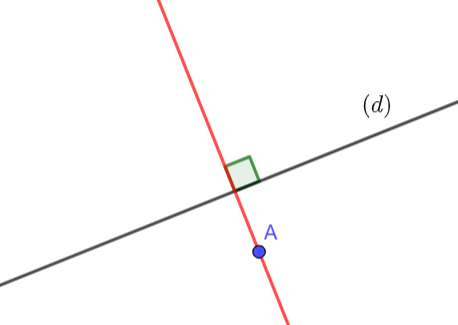
\includegraphics[width=0.5\linewidth]{../../assets/images/6e/seq_02/point_droite_perpendiculaire}
\end{center}
\vspace{0.5cm}

\textit{Que le point A soit sur la droite (d) ou à l'extérieur, il n'y a toujours qu'une seule façon de tracer la perpendiculaire passant par A.}
\end{proprietebox}

\section*{6) Application : Lire attentivement une consigne}

\noindent
La différence entre les articles \og un/une \fg{} et \og le/la \fg{} est cruciale en géométrie. 
Elle indique si le tracé est unique ou si vous avez le choix !

\vspace{0.5cm} % Ajoute un petit espace vertical

\begin{itemize}
	\item \textbf{Tracer \underline{la} droite (AB)} : il n'y a qu'\textbf{\textcolor{red}{une seule possibilité}}. Les points A et B sont connus.
	
	\item \textbf{Tracer \underline{une} droite parallèle à la droite (d)} : il y a une \textbf{\textcolor{red}{infinité de possibilités}}. On peut tracer n'importe laquelle.
	
	\item \textbf{Tracer \underline{la} droite parallèle à la droite (d) passant par B} : cette droite est \textbf{\textcolor{red}{unique}}. Il n'y a qu'un seul tracé qui répond à cette consigne.
	
	\item \textbf{Tracer \underline{une} droite (d)} : il y a une \textbf{\textcolor{red}{infinité de possibilités}}. On peut tracer cette droite comme on le souhaite.
	
	\item \textbf{Tracer \underline{le} cercle de centre O et de rayon 4~cm} : ce cercle est \textbf{\textcolor{red}{unique}}. Il n'y a qu'un seul tracé qui répond à cette consigne.
\end{itemize}

% =========================
\section{ Je m'entraîne}
\begin{itemize}
	\item Lecture : $[MN]$: \trous{12cm}\\
	 $(RS)$: \trous{12cm}\\
	 $[TU)$: \trous{12cm}\\
	 $VU$: \trous{12cm}
	\item Notations : << La droite passant par $P$ et $Q$ >>: \trous{12cm}\\
	 << Le segment d'extrémités $K$ et $L$ >>: \trous{12cm} \\
	 << La demi-droite d'origine $H$ passant par $J$ >>: \trous{12cm} \\
	 << La longueur du segment d'extrémités A et B >>: \trous{12cm}
	\item Complète : Si $A \in (BC)$ alors $A,B,C$ sont \trou{3cm}. Si $D \notin (EF)$ alors D, E et F ......................................
\end{itemize}
